\documentclass{amsart}
\usepackage{graphicx}
\graphicspath{{./}}
\usepackage{hyperref}
\usepackage{csvsimple}
\usepackage{longtable}
\usepackage{epigraph}
\title{Calibration of Zulf's Markov Moral Theory for Human Race To Error 0.817}
\author{Zulfikar Moinuddin Ahmed}
\date{\today}
\begin{document}
\maketitle

\section{A Historical Perspective}
Between Black-Scholes-Merton's first models in the early 1970s to long memory stochastic volatility models such as mine from 2018, close to 50 years had passed. This is the timescale for refined quantitative scientific models to reach maturity.  We are not blind to the process; what we are able to see of Human Moral Nature with our current model of Markov Homogeneity will reach maturity with refinements and clarity that is impossible for us to predict.  Nevertheless our Markov Moral model is pioneering and successful, much like the Black-Scholes-Merton early model was.  We have made a phase transition from purely humanistic and theological considerations about Moral Nature of Man to quantitative models.  

This note presents a solid success.  We are fitting 55 free parameters of a transition density $P$ that is $10 \times 10$.  Our assumption is perfect homogeneity of all morals, and we are simultaneously fitting 15 vectors in $\mathbf{R}^{10}$.  For this, the minimum error of fit being $\varepsilon=0.817$ is quite good.  It is not zero, and thus we have a good but imperfect model.  

\begin{verbatim}
# load data
wvs7<-readRDS("wvs7.rds")
vars<-c("Q290","Q46", "Q57","Q177","Q178","Q179","Q180","Q181","Q182","Q183","Q184","Q185","Q186","Q187","Q188","Q189","Q190","Q191","Q192","Q193","Q194","Q195","Q275","Q192")

# Create ethnicity table 
# by mapping various detailed
# country-based ethnicities to
# broader groups
library(haven)
# Problem is WVS Q290 has too many 
# gradations when we want to deal 
# with a few classes that can allow 
# us to overcome ethnic prejudices
ethnicities<-unique(as.character(as_factor(wvs7$Q290)))

reduced_ethnicities<-function(){
  mapeth<-rep("Other",length(ethnicities))
  mapeth[c(1,7,15,33,38,43,65,107,154,210,214)]<-"White"
  mapeth[c(3,223,222,51,52,53,54,55,56,45,39,36,11)]<-"Black"
  mapeth[c(6,13,19,20,21,22,67,70)]<-"Indian"
  mapeth[c(4,17,48,97,98,99,100)]<-"Arab"
  mapeth[c(5,14,16,62,63,64,68,72,73,74,75,76,77,
           78,79,80,81,82,83)]<-"East Asian"
  data.frame(key=ethnicities,val=mapeth)
}

ethnicity_map<-function( v ){
  emap<-reduced_ethnicities()
  w<-sapply(as.character(as_factor(v)),function(x) { out<-emap[which(emap$key==x),]$val; if(is.null(out)){out<-"Other"};return(out)})
  #print(head(w))
  #w<-append(w,"Other")
  as.factor(unlist(w))
}



polv<-na.omit(wvs7[,vars])
polv$eth<-ethnicity_map(as_factor(polv$Q290))

# Fit P to distributions to Q177-Q195 in WVS 7
library(markovchain)

t10 <-1:10
nrm<-function(v)v/sum(v)

transitionMatrixFromPars<-function(x){
  P<-matrix(0,nrow=10,ncol=10)
  P[1,1]<-x[1]
  P[1:2,2]<-x[2:3]
  P[1:3,3]<-x[4:6]
  P[1:4,4]<-x[7:10]
  P[1:5,5]<-x[11:15]
  P[1:6,6]<-x[16:21]
  P[1:7,7]<-x[22:28]
  P[1:8,8]<-x[29:36]
  P[1:9,9]<-x[37:45]
  P[1:10,10]<-x[46:55]
  #symmetrize
  for (k in 2:10){
    P[k,1:k]<-P[1:k,k]
  }
  for (k in 1:10){
    P[k,]<-nrm(P[k,])
  }
  P
}

parsFromTransitionMatrix<-function(P){
  x<-c()
  for (k in 1:10){
    x<-append(x, P[1,1:k])
  }
  x
}

# We let x be the parameters of the subdiagonal
# of P in form appropriate for an optimiser
moral_markov_obj<-function( x ){
  
  P <- transitionMatrixFromPars( x )
  states <- as.character(1:10)
  mcVals = new("markovchain", 
               states = states,
               transitionMatrix = P,          
               name = "Vals")
  Imtx <- matrix( 0, nrow=18,ncol=10)
  Jmtx <- matrix( 0, nrow=18, ncol=10)
  I4<-nrm(table(polv[,"Q180"]))
  Imtx[4,] <- I4
  M<-10000
  Y1<-sample(1:10,M,replace=TRUE,prob=I4)
  all.Y<-matrix(0,nrow=M,ncol=18)
  all.Y[,4]<-Y1
  for (kk in 1:M) {
    #print(kk)
    outs <- rmarkovchain(n = 18, object = mcVals, what = "list")
    all.Y[kk,1:18]<-outs  
  }

  for ( r in 1:18 ){
    iv<-nrm(table(polv[,vars[r]]))
    jv<-nrm(table(all.Y[,r]))
    ivn<-rep(0,10)
    jvn<-rep(0,10)
    for ( kc in 1:10 ){
      a<-iv[as.character(kc)]
      b<-jv[as.character(kc)]
      if (!is.null(a)){
          ivn[kc]<-a
      }
      if (!is.null(b)){
        jvn[kc]<-b
      }
        
    }
    Imtx[r,]<-ivn
    Jmtx[r,]<-jvn
  }

  print('calculating l2 distance')  
  l2.dist <- 0
  hits<-0
  for (r in 1:18){
    d1<- norm(abs(Imtx[r,]),type="2")
    d2<- norm(abs(Jmtx[r,]),type="2")
    d <- norm( abs(Imtx[r,] - Jmtx[r,] ), type="2")
    #print(paste("r=",r,"d1=",d1,"d2=",d2,"d=",d))
    if (!is.na(d)){
      hits<-hits+1
      l2.dist <- l2.dist + d^2
    }
  }
  l2.dist<-sqrt(l2.dist)
  print(paste('hits=',hits))
  print(l2.dist)
  l2.dist
}




library(nloptr)
# Get an init value
lambda <- 0.52
p11 <- 0.6
P <- matrix(0,nrow = 10, ncol=10)
P[1,1] = p11
for (k in 2:10){
  for (r in 1:k){
    P[k,r] <- exp(-lambda*(k+r))*p11
    P[r,k] <- P[k,r]
  }
}
for ( r in 1:10){
  P[r,]<-P[r,]/sum(P[r,])
}
P0<-P

x0<-parsFromTransitionMatrix(P0)
xlen <- length(x0)
l0 <- rep(0,xlen)
u0 <- rep(1,xlen)

eval_g0<-function( x ){
  P1<-transitionMatrixFromPars(x)
  out<-0
  for (k in 1:10){
    out <- out + (sum(P1[k,]))^2-1.0
  }
  out
}

# Solve using NLOPT_LN_COBYLA without gradient information
res1 <- nloptr( x0=x0,
                eval_f=moral_markov_obj,
                lb = l0,
                ub = u0,
                opts = list("algorithm"="NLOPT_LN_NELDERMEAD",
                            "xtol_rel"=1.0e-6,
                            "maxeval"=5000,
                            "print_level"=1))
print( res1 )
\end{verbatim}

\section{Results}

\begin{verbatim}
Call:

nloptr(x0 = x0, eval_f = moral_markov_obj, lb = l0, ub = u0, 
    opts = list(algorithm = "NLOPT_LN_NELDERMEAD", xtol_rel = 1e-06, 
        maxeval = 5000, print_level = 1))


Minimization using NLopt version 2.4.2 

NLopt solver status: 4 ( NLOPT_XTOL_REACHED: Optimization 
stopped because xtol_rel or xtol_abs (above) was reached. )

Number of Iterations....: 1783 
Termination conditions:  xtol_rel: 1e-06	maxeval: 5000 
Number of inequality constraints:  0 
Number of equality constraints:    0 
Optimal value of objective function:  0.817045481661292 
Optimal value of controls: 0.9296093 0.9461727 0.1329849 0.9528866 0.1232481 0.1840176 
0.7054217 0.1208542 0.07592334 0.04760389 0.9743768 0.1271022 
0.05002236 0.05245708 0.07770686 0.6887877 0.1204812 
0.08294907 0.0494034 0.02994026 0.01768977 0.9798776 
0.1242425 0.08783196 0.05152778 0.03319163 0.03989205 
0.01110893 0.71306 0.1256979 0.0816829 0.04975205 0.02954562 
0.01829363 0.01137643 0.007001064 0.6999624 0.1279634 
0.08883094 0.05064857 0.03351747 0.01924939 0.005506017 
0.006374397 0.003926346 0.7152188 0.1291862 0.08420505 
0.05199877 0.03114507 0.0197665 0.01128659 0.007152566 
0.004032615 0.002253443
\end{verbatim}

\section{Tabular Display of fitted $P$}

% latex table generated in R 4.0.3 by xtable 1.8-4 package
% Wed May  5 21:29:42 2021
\begin{table}[ht]
\centering
\begin{tabular}{rrrrrrrrrrr}
  \hline
 & 1 & 2 & 3 & 4 & 5 & 6 & 7 & 8 & 9 & 10 \\ 
  \hline
1 & 11.19 & 11.39 & 11.47 & 8.49 & 11.73 & 8.29 & 11.80 & 8.59 & 8.43 & 8.61 \\ 
  2 & 45.53 & 6.40 & 5.93 & 5.82 & 6.12 & 5.80 & 5.98 & 6.05 & 6.16 & 6.22 \\ 
  3 & 52.60 & 6.80 & 10.16 & 4.19 & 2.76 & 4.58 & 4.85 & 4.51 & 4.90 & 4.65 \\ 
  4 & 56.18 & 9.63 & 6.05 & 3.79 & 4.18 & 3.93 & 4.10 & 3.96 & 4.03 & 4.14 \\ 
  5 & 67.71 & 8.83 & 3.48 & 3.65 & 5.40 & 2.08 & 2.31 & 2.05 & 2.33 & 2.16 \\ 
  6 & 63.40 & 11.09 & 7.63 & 4.55 & 2.76 & 1.63 & 3.67 & 1.68 & 1.77 & 1.82 \\ 
  7 & 72.27 & 9.16 & 6.48 & 3.80 & 2.45 & 2.94 & 0.82 & 0.84 & 0.41 & 0.83 \\ 
  8 & 67.91 & 11.97 & 7.78 & 4.74 & 2.81 & 1.74 & 1.08 & 0.67 & 0.61 & 0.68 \\ 
  9 & 67.30 & 12.30 & 8.54 & 4.87 & 3.22 & 1.85 & 0.53 & 0.61 & 0.38 & 0.39 \\ 
  10 & 67.71 & 12.23 & 7.97 & 4.92 & 2.95 & 1.87 & 1.07 & 0.68 & 0.38 & 0.21 \\ 
   \hline
\end{tabular}
\end{table}

\section{Residuals}

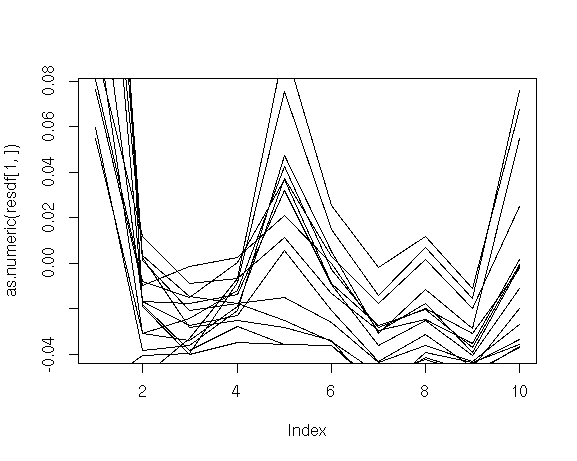
\includegraphics[scale=0.8]{markovmoralserr.jpeg}

Size of errors (in $\mathbf{R}^{10}$ ).

\begin{verbatim}
> for(k in 1:15){print(sqrt(sum(resdf[k,]^2)))}
[1] 0.09562637
[1] 0.1103395
[1] 0.3569231
[1] 0.2358779
[1] 0.3081056
[1] 0.1180627
[1] 0.1582781
[1] 0.1314817
[1] 0.165995
[1] 0.1362075
[1] 0.2384125
[1] 0.0907127
[1] 0.3603582
[1] 0.1037558
[1] 0.2911007
\end{verbatim}

\end{document}
